\documentclass[11pt]{article}

\usepackage{amsmath}
\usepackage{amssymb}
\usepackage{amsthm}
\usepackage{hyperref}
\usepackage{ulem}
\usepackage{enumitem}
\usepackage[left=0.75in, right=0.75in, bottom=0.75in]{geometry}
\usepackage{graphicx}
\usepackage{float}

\usepackage{chngcntr}
\counterwithin*{equation}{section}
\counterwithin*{equation}{subsection}

\usepackage{fancyhdr}
\pagestyle{fancy}
\fancyhf{}
\lhead{190100044 \& 190100055}
\rhead{CS 215: Assignment 1}
\renewcommand{\footrulewidth}{1.0pt}
\cfoot{Page \thepage}

\setlength{\parindent}{0em}

\title{Assignment 1: CS 215}
\author{190100044 \& 190100055}
\date{31st August 2020}

\begin{document}

\maketitle
\tableofcontents
\thispagestyle{empty}
\setcounter{page}{0}



\newpage
\section*{Question 1}
\addcontentsline{toc}{section}{Question 1}
\begin{enumerate}[label=(\alph*)]
    \item The probability that the first person picks up his/her own book is $\frac{1}{n}$, for the second person, there are $n-1$ books remaining, thus the probability for him/her is $\frac{1}{n-1}$, similarly, the $i^{th}$ person has $ (n-i+1) $ choices, out of which $1$ is correct, thus $P(E_i)$, the probability that the $i^{th}$ person picks up his/her own book is given by: $\frac{1}{n-i+1}$.\\
          Thus, the probability that each person picks up his/her own book ($ \cap_{i=1}^{n} P(E_i) $) is given by:
          $$ \prod_{i=1}^n \Big( \frac{1}{n-i+1} \Big) = \frac{1}{n!}$$
          Alternative:\\
          $N(\text{Sample space}) = n!$ and only one unique permutation is possible such that every person picks his/her book. Therefore,
          $$ P(E) = \frac{1}{n!} $$

    \item Similar to the previous case, we have, the probability that the first $ m < n $ persons who picked up a book receive their own book back again ($ \cap_{i=1}^{m} P(E_i) $),
          $$ \prod_{i=1}^m \Big( \frac{1}{n-i+1} \Big) = \frac{(n-m)!}{n!} $$

    \item The first person to pick a book now has $m$ correct choices out of $n$, similarly, the second person has $m-1$ correct choices out of $n-1$ books. Thus, the $i^{th}$ person ($ i \le m $) has $ (m-i+1) $ correct choices, out of $(n-i+1)$ choices. Thus $P(E_i)$, the probability that the $i^{th}$ person ($i < m$) gets back a book belonging to \textbf{one} of the last $m$ persons is equal to: $\frac{m-i+1}{n-i+1}$.\\
          Thus, the probability that each person among the first $m$ persons to pick up the book gets back a book belonging to one of the last $m$ persons to pick up the books is: ($ \cap_{i=1}^{m} P(E_i) $)
          $$ \prod_{i=1}^m \Big( \frac{m-i+1}{n-i+1} \Big) = \frac{m!(n-m)!}{n!} $$

    \item The first $m$ persons can pick up any book and each book needs to be clean. Thus $P(E_i)$, the probability that the $i^{th}$ person picks up a book which is clean, is equal to $(1-p)$.\\
          Thus, the probability that each person among the first $m$ persons picks up a clean book is: ($ \cap_{i=1}^{m} P(E_i) $)
          $$ (1-p)^m $$

    \item Exactly $m$ persons\footnote{Note that these $m$ persons \textbf{may not} be the first $m$ persons} need to pick up a clean book.\\
          Thus, the ways to choose $m$ persons out of $n$ is ${n\choose m}$, all these chosen people must have chosen a clean book (probability: ($1-p$)), while all the ($ n-m $) remaining people must choose an unclean book (probability: $p$), since it is mentioned \textbf{\textit{exactly}} $m$ persons must choose a clean book.\\
          Thus this probability is given by:
          $$ {n\choose m} (1-p)^m (p)^{n-m} $$

\end{enumerate}



\newpage
\section*{Question 2}
\addcontentsline{toc}{section}{Question 2}
By the definition of the variance\footnote{Note: Here $\sigma$ is defined to be the \textbf{positive} square root of the variance}, $\sigma^2$, we have:
$$ \sigma^2 = \frac{\sum_{i=1}^n (x_i - \mu)^2}{n-1} $$
\begin{equation}
    \label{var}
    (n-1)\sigma^2 = \sum_{i=1}^n (x_i - \mu)^2
\end{equation}
Since $(x_i - \mu)^2 \ge 0 \  \forall \ i$, we have ((for all $i$)):
$$ \sum_{i=1}^n (x_i - \mu)^2 \ge (x_i - \mu)^2  $$
Thus, by (\ref{var}) we get (for all $i$):
$$ (n-1)\sigma^2 \ge (x_i - \mu)^2 $$
Taking the square root on both sides,
$$ \sigma\sqrt{n-1} \ge |x_i - \mu| \implies |x_i - \mu| \le \sigma\sqrt{n-1} \hfill $$
\hfill \qedsymbol \\
\noindent
The (Two-sided) Chebyshev's inequality states that:
$$ |S_k| = \{ x_i : \  |x_i - \mu| \ge k\sigma \} $$
\begin{equation}
    \frac{|S_k|}{n} < \frac{1}{k^2}
\end{equation}
Consider $k = \sqrt{n-1}$ in the above equation,\\
$$ |S_{\sqrt{n-1}}| = \{ x_i : \  |x_i - \mu| \ge \sigma\sqrt{n-1} \} $$
$$ \frac{|S_{\sqrt{n-1}}|}{n} < \frac{1}{n-1} $$
$$ 0 \leq |S_{\sqrt{n-1}}| < \frac{n}{n-1}$$
$$ \lim_{n\to\infty}0=0 \leq \lim_{n\to\infty}|S_{\sqrt{n-1}}| < \lim_{n\to\infty}\bigg( \frac{n}{n-1} \bigg)=1$$
Thus,
$$ \lim_{n\to\infty}|S_{\sqrt{n-1}}| = 0 $$
The inequality proven earlier also says that $\forall i \ |x_i - \mu| \le \sigma \sqrt{n-1}$, i.e. $|S_{\sqrt{n-1}}| = 0$.\\



\newpage
\section*{Question 3}
\addcontentsline{toc}{section}{Question 3}
We have,
\begin{equation*}
    \begin{split}
        \mu &= \frac{\sum_{i=1}^n x_i}{n} \\
        \mu - \tau &= \frac{\sum_{i=1}^n x_i}{n} - \tau \\
            &= \frac{(\sum_{i=1}^nx_i) - n\tau}{n} \\
            &= \frac{\sum_{i=1}^n (x_i - \tau)}{n}
    \end{split}
\end{equation*} 
\begin{equation}
    \label{res1}
    |\mu - \tau| = \Bigg|\frac{\sum_{i=1}^n (x_i - \tau)}{n}\Bigg| \le \frac{\sum_{i=1}^n |x_i - \tau|}{n}
\end{equation}
We also know that the median minimizes the total absolute deviation.
\begin{equation*}
    \sum_{i=1}^n |x_i - \tau| \le \sum_{i=1}^n |x_i - y| \hspace{2em} \forall \ y 
\end{equation*}
Let $y = \mu$, thus we get:
\begin{equation*}
    \sum_{i=1}^n |x_i - \tau| \le \sum_{i=1}^n |x_i - \mu|
\end{equation*}     
By \eqref{res1}, and the above result, we have:
\begin{equation}
    \label{res2}
    |\mu - \tau| \le \frac{\sum_{i=1}^n |x_i - \tau|}{n} \le \frac{\sum_{i=1}^n |x_i - \mu|}{n}
\end{equation}
We also have:
\begin{equation}
    \label{res3}
    \begin{split}
        \sigma &= \sqrt{\frac{\sum_{i=1}^n (x_i - \mu)^2}{n-1}} \\
            &> \sqrt{\frac{\sum_{i=1}^n (x_i - \mu)^2}{n}} \ge \frac{\sum_{i=1}^n |x_i - \mu|}{n} \hspace{2em} \\
            &\text{(Root Mean Square $\ge$ Arithmetic Mean)}
    \end{split}
\end{equation}
Therefore from \eqref{res2} and \eqref{res3}, we get that
\begin{equation*}
    |\mu - \tau| \le \sigma
\end{equation*}
% TODO: Show R.H.S is less than equal to $\sigma$



\newpage
\section*{Question 4}
\addcontentsline{toc}{section}{Question 4}
Let $A$ be the event that the rickshaw is red.\\
Thus, as a given rickshaw must be either red or blue, $A^c$ is the event that the rickshaw is blue.\\
Let $B$ be the event that the rickshaw is observed as red by the person under the given conditions.\\
We have been given the following:
$$
    P(A) = \frac{1}{100} \implies P(A^c) = \frac{99}{100}
$$
$$
    P(B|A) = 0.99 \ \  P(B|A^c) = 0.02
$$
We need to find $P(A|B)$. \\
\\
We shall first find $P(B)$,
$$
    \begin{aligned}
        P(B) & = P(B|A)P(A) + P(B|A^c)P(A^c)     \\
             & = 0.99\times0.01 + 0.02\times0.99 \\
             & = 0.0297
    \end{aligned}
$$
\\
Now, by Bayes Theorem,
$$
    \begin{aligned}
        P(A|B) & = \frac{P(B|A)P(A)}{P(B)}            \\
               & = \frac{0.99\times0.01}{0.0297}      \\
               & = \frac{1}{3} = 0.33 = \mathbf{33\%}
    \end{aligned}
$$
Thus, the defence lawyer can argue that there was only a $33\%$ chance that the rickshaw observed by the person XYZ was indeed red.



\newpage
\section*{Question 5}
\addcontentsline{toc}{section}{Question 5}
\begin{enumerate}[label=(\alph*)]
    \item
          Event of choosing a door is independent of which door contains the car as the contestant is unaware of the car's location. Therefore, $C_i$ and $Z_i$ are independent events.
          \begin{equation*} \label{eq1}
              \begin{split}
                  P(C_i|Z_1) &= P(C_i) \hspace{3em} \forall i \in {1, 2, 3} \\
                  &= \mathbf{\frac{1}{3}} \hspace{5em} \forall i \in {1, 2, 3}
              \end{split}
          \end{equation*}

    \item
          Keeping in mind, the fact given about the intelligence of the host, we can produce following conclusions.\\
          If $(C_1, Z_1)$ happen, then the host has equal chances of choosing Door 2 and Door 3, therefore,
          \begin{align*}
              P(H_1|C_1,Z_1) & = 0 & P(H_2|C_1,Z_1) & = \frac{1}{2} & \mathbf{P(H_3|C_1,Z_1)} & = \mathbf{\frac{1}{2}}
          \end{align*}
          If $(C_2, Z_1)$ happen, then the host will open Door 3, therefore,
          \begin{align*}
              P(H_1|C_2,Z_1) & = 0 & P(H_2|C_2,Z_1) & = 0 & \mathbf{P(H_3|C_2,Z_1)} & = \mathbf{1}
          \end{align*}
          If $(C_3, Z_1)$ happen, then the host will open Door 2, therefore,
          \begin{align*}
              P(H_1|C_3,Z_1) & = 0 & P(H_2|C_3,Z_1) & = 1 & \mathbf{P(H_3|C_3,Z_1)} & = \mathbf{0}
          \end{align*}

    \item
          \begin{align*}
              \begin{split}
                  P(H_3, Z_1) &= P(H_3 \cap (C_1 \cup C_2 \cup C_3) \cap Z_1) \\
                  &= P((H_3 \cap (C_1 \cap Z_1)) \cup (H_3 \cap (C_1 \cap Z_1)) \cup (H_3 \cap (C_1 \cap Z_1))) \\
                  &= P(H_3|C_1,Z_1) \cdot P(C_1,Z_1) + P(H_3|C_2,Z_1) \cdot P(C_2,Z_1) + P(H_3|C_2,Z_1) \cdot P(C_2,Z_1) \\
                  &= \frac{1}{2} \cdot \frac{1}{9} + 1 \cdot \frac{1}{9} + 0 \cdot \frac{1}{9} \\
                  &= \frac{1}{6}
              \end{split} \\\\
              \begin{split}
                  P(C_2|H_3, Z_1) &= \frac{P(H_3|C_2, Z_1) \cdot P(C_2, Z_1)}{P(H_3, Z_1)} \\
                  &= \frac{1 \cdot \frac{1}{9}}{\frac{1}{6}} \\
                  &= \frac{2}{3} \\
                  &= \mathbf{67\%}
              \end{split}
          \end{align*}

    \item
          $P(H_3|C_3,Z_1) = 0 \implies P(C_3|H_3, Z_1)=0$ \hspace{1em} (Host is intelligent)\\
          Therefore, $P(C_1|H_3, Z_1) = 1 - P(C_2|H_3, Z_1) = \frac{1}{3} = \mathbf{33\%}$

    \item
          $P(C_2|H_3, Z_1) > P(C_1|H_3, Z_1)$, i.e., the chances of winning the car is higher if the contestant switches his/her choice.

    \item
          Now, that the intelligence of the host is compromised.\\
          If $(C_i, Z_1)$ happen for any i, then the host has equal chances of choosing Door 2 and Door 3, therefore,
          \begin{align*}
              P(H_1|C_i,Z_1) & = 0 & P(H_2|C_i,Z_1) & = \frac{1}{2} & P(H_3|C_i,Z_1) & = \frac{1}{2} \hspace{3em} \forall i \in {1, 2, 3}
          \end{align*}
          \begin{align*}
              \begin{split}
                  P(H_3, Z_1) &= P(H_3|C_1,Z_1) \cdot P(C_1,Z_1) + P(H_3|C_2,Z_1) \cdot P(C_2,Z_1) + P(H_3|C_2,Z_1) \cdot P(C_2,Z_1) \\
                  &= \frac{1}{2} \cdot \frac{1}{9} + \frac{1}{2} \cdot \frac{1}{9} + \frac{1}{2} \cdot \frac{1}{9} \\
                  &= \frac{1}{6}
              \end{split} \\\\
              \begin{split}
                  P(C_2|H_3, Z_1) &= \frac{P(H_3|C_2, Z_1) \cdot P(C_2, Z_1)}{P(H_3, Z_1)} \\
                  &= \frac{\frac{1}{2} \cdot \frac{1}{9}}{\frac{1}{6}} \\
                  &= \frac{1}{3} \\
              \end{split}
          \end{align*}
          Similarly, $P(C_1|H_3, Z_1) = P(C_3|H_3, Z_1) = \frac{1}{3}$\\
          Now, if the Door 3 contains the car and it is shown to the contestant, then the contestant can simply choose that door (if allowed).\\
          Else the contestant has equal probability to win a car with and without switching to Door 2.

\end{enumerate}



\newpage
\section*{Question 6}
\addcontentsline{toc}{section}{Question 6}
\begin{figure}[H]
    \centering
    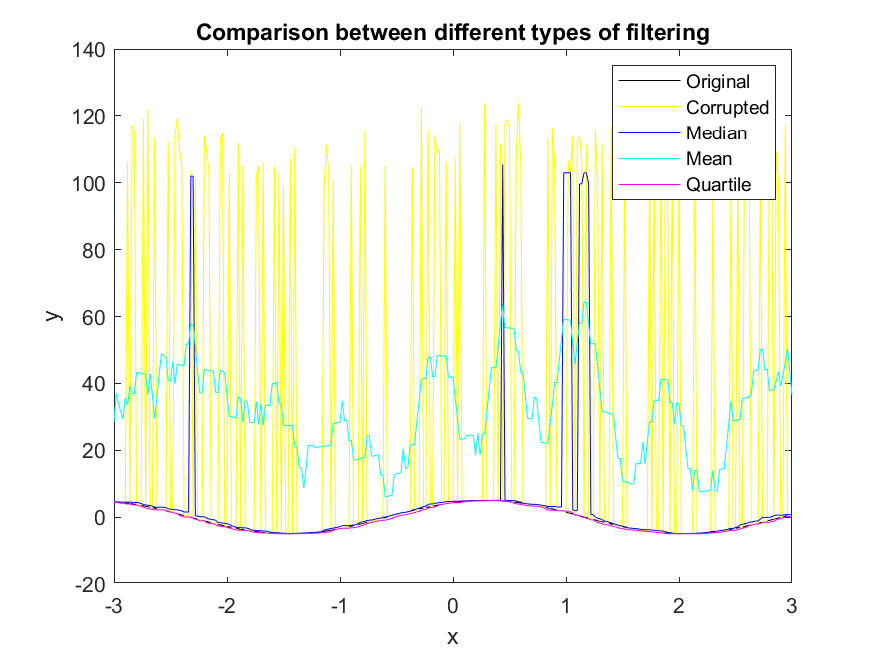
\includegraphics[scale=0.9]{q6.1.png}
\end{figure}
\begin{figure}[H]
    \centering
    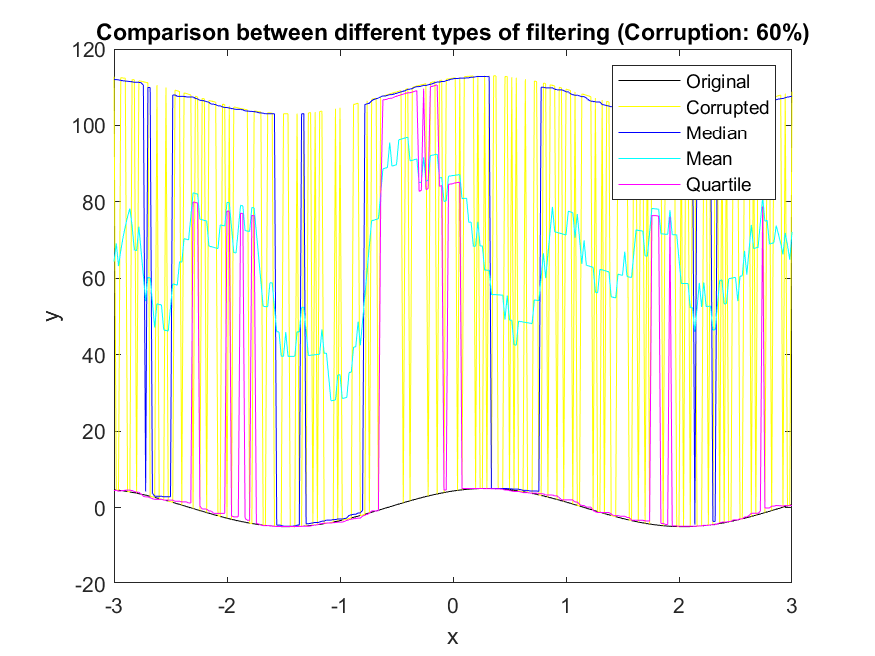
\includegraphics[scale=0.9]{q6.2.png}
\end{figure}
\begin{center}
    \begin{tabular}{|c|c|c|}
        \hline
        \textbf{Results} & \textbf{Mean Square Error (30\% Corruption)} & \textbf{Mean Square Error (60\% Corruption)} \\
        \hline
        Corrupted        & 266.09                                       & 588.35                                       \\
        \hline
        Median           & 26.52                                        & 372.31                                       \\
        \hline
        Mean             & 90.15                                        & 737.09                                       \\
        \hline
        Quartile         & 0.01                                         & 117.38                                       \\
        \hline
    \end{tabular}
\end{center}

\textbf{Quartile} method produced the best relative mean squared error.
\subsection*{Explanation:}
Let's choose an arbitrary window $W$ of length $w$ (in our case, $w$=17)
$$ W := \{ x_1, x_2, \ldots, x_w \} $$
Assume that the values in $W$ are sorted.\\
Let the median be (approximately) at position $m$\\
Let the first quartile be (approximately) at position $q$\\
After corruption, let $n_c$ values out of these $w$ get corrupted.

\medskip
\textbf{Assumption:} After corruption, the values can only increase. (Note that this is true for our case as we are adding values in the range 100 to 120)\\
\textbf{Case Q:}\\
For quartile to change after corruption, \textbf{at least} $1$ value before $x_q$ must get corrupted (Let this be Event Q).\\
\textbf{Case M:}\\
For median to change after corruption, \textbf{at least} $1$ value before $x_m$ must get corrupted (Let this be Event M).\\
\\
As the amount of corruption increases, the probabilities of \textbf{both} these cases increase, but as $m > q$, the probability that Event M occurs is always more than the probability that Event Q occurs.\\
Thus, the relative mean squared error is always smaller for quartile filtering as compared to median filtering.\\

\medskip
\textbf{For mean:}\\
Even if a single value, anywhere in the data, gets corrupted, then mean will change drastically. Thus the relative mean squared error is always the highest for mean filtering as compared to quartile and median filtering.



\newpage
\section*{Question 7}
\addcontentsline{toc}{section}{Question 7}

\subsection*{Mean}
Given $n$ values $\{x_i\}^n_{i=1}$ having mean $\mu$.\\
Now we add $x_{n+1}$ to the set. Let the new mean be $\mu'$.
\begin{equation*}
    \begin{split}
    \mu &= \frac{\sum_{i=1}^{n} x_i}{n} \\
    \sum_{i=1}^{n} x_i &= n\mu \\
    \sum_{i=1}^{n+1} x_i &= n\mu + x_{n+1} \\
    \mu' &= \frac{\sum_{i=1}^{n+1} x_i}{n+1} \\
        &= \frac{n\mu + x_{n+1}}{n+1} \\
        &\approx \mu + \frac{x_{n+1}}{n} \hspace{2em} \text{(Given n is large)} \\
    \end{split}
\end{equation*}

\subsection*{Median}
Given sorted $n$ values $\{x_i\}^n_{i=1}$ having median $\tau$. \\
Now we add $x'$ to the set. Let the new median be $\tau'$. \\

For even $n$,
\begin{center}
$\tau = \frac{x_{\frac{n}{2}} + x_{\frac{n}{2}+1}}{2}$.\\
$x' < x_{\frac{n}{2}} \implies \tau' = x_{\frac{n}{2}}$ \\
$x_{\frac{n}{2}} < x' < x_{\frac{n}{2}+1} \implies \tau' = x'$ \\
$x_{\frac{n}{2}+1} < x' \implies \tau' = x_{\frac{n}{2}+1}$ \\
\end{center}

For odd $n$,
\begin{center}
$\tau = x_{\frac{n+1}{2}}$ \\
$x' < x_{\frac{n-1}{2}} \implies \tau' = \frac{x_{\frac{n-1}{2}} + x_{\frac{n+1}{2}}}{2}$ \\
$x_{\frac{n-1}{2}} < x' < x_{\frac{n+1}{2}} \implies \tau' = \frac{x' + x_{\frac{n+1}{2}}}{2}$ \\
$x_{\frac{n+1}{2}} < x' < x_{\frac{n+3}{2}} \implies \tau' = \frac{x_{\frac{n+1}{2}} + x'}{2}$ \\
$x_{\frac{n+3}{2}} < x' \implies \tau' = \frac{x_{\frac{n+1}{2}} + x_{\frac{n+3}{2}}}{2}$
\end{center}

\subsection*{Standard Deviation}
Given $n$ values $\{x_i\}^n_{i=1}$ having mean $\mu$ and standard deviation $\sigma$. \\
Now we add $x_{n+1}$ to the set. Let the new mean $\mu'$ and new standard deviation $\sigma'$. \\
\begin{equation*}
    \begin{split}
        \sigma^2 &= \frac{\sum_{i=1}^{n} (x_i - \mu)^2}{n-1} \\
            &= \frac{\sum_{i=1}^{n} (x_i)^2 - 2\mu\sum_{i=1}^{n} (x_i) + n\mu^2 }{n-1} \\
            &= \frac{\sum_{i=1}^{n} (x_i)^2 - 2\mu\cdot(n\mu) + n{\mu}^2}{n-1} \\
            &= \frac{\sum_{i=1}^{n} (x_i)^2 - n{\mu}^2}{n-1} \\
    \end{split}
\end{equation*}
\begin{equation*}
    \begin{split}
        \sum_{i=1}^{n} (x_i)^2 &= (n-1)\sigma^2 + n{\mu}^2 \\
        \sum_{i=1}^{n+1} (x_i)^2 &= \sum_{i=1}^{n} (x_i)^2 + x_{n+1}^2 \\
            &= (n-1)\sigma^2 + n{\mu}^2 + x_{n+1}^2 \\
        \sigma'^2 &= \frac{\sum_{i=1}^{n+1} (x_i)^2 - n{\mu'}^2}{n} \\
            &= \frac{(n-1)\sigma^2 + n{\mu}^2 + x_{n+1}^2 - n{\mu'}^2}{n} \\
            &\approx \sigma^2 + \mu^2 - \mu'^2 + \frac{x_{n+1}^2}{n} \hspace{2em} \text{(Given n is large)} \\
    \end{split}
\end{equation*}


\end{document}

